\chapter{Auswertung} \label{Auswertung}

Im folgenden Kapitel wird die Auswertung anhand der in Kapitel \ref{Bewertungskriterien} aufgestellten Bewertungskriterien beschrieben. Zu den einzelnen Kategorien wird der jeweilige ausgefüllte Abschnitt der Bewertungsmatrix dargestellt und erläutert. 

\section{Kosten und Lizenz}

Nachfolgende Abbildung \ref{fig:AuswKostLiz} zeigt den Abschnitt 'Kosten und Lizenz' der ausgefüllten Bewertungsmatrix.

\begin{figure}[h]
	\centering
	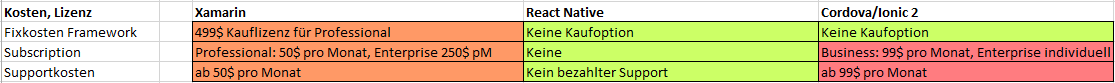
\includegraphics[width=1\textwidth]{Bilder/Auswertung_KostenLizenz.PNG}
	\caption{Bewertungsmatrix Kategorie Kosten und Lizenz}
	\label{fig:AuswKostLiz}
\end{figure}

Das Xamarin Framework gibt es in einer kostenlosen Community-Version und in den kostenpflichtigen Versionen 'Professional' und 'Enterprise'. Die kostenlose Community-Version gibt es für Windows inklusive einer Community-Version von Visual Studio und für Apple mit der IDE 'Xamarin Studio'. Die Preise der kostenpflichtigen Versionen richten sich nach den Preisen der entsprechenden Version der IDE Visual Studio. Die Professional-Version kann für 499\$ ohne Subscription oder für 1199\$ mit Subscription erworben werden. Eine Subscription hält 2 Jahre, ein Auffrischen danach kostet 799\$. Die Enterprise-Version kann nur mit Subscription erworben werden. Sie kostet 5999\$ und ein Auffrischen nach Ablauf der 2 Jahre kostet 2569\$. Einen technischer Support  erhält man mit jeder Subscription, das bedeutet ab umgerechnet 50\$ pro Monat. E-Mail-Support erhalten alle Business- und Enterprise-Kunden. Zusätzlich zu allen Modellen kann die Xamarin Test-Cloud ab einen monatlichen Preis von 99\$ genutzt werden\footcite{XamarinPricing}.
\\
\\
Für das Framework React Native gibt es keine kostenpflichtigen Versionen\footcite{ReactNativeHomepage}. 
\\
\\
Für das Framework Cordova gibt es ebenfalls keine kostenpflichtigen Modelle. Das Framework Ionic bietet dagegen folgende Varianten an: eine kostenlose Community-Version und die kostenpflichtigen Versionen 'Indie', 'Business' und 'Enterprise'. Im Gegensatz zu den kostenpflichtigen Modellen bei Xamarin, fallen bei den Modellen von Ionic monatliche Subscription-Gebühren an. Die Indie-Variante kostet 25\$ pro Monat und die Business-Variante kostet 99\$ pro Monat. Für die Enterprise-Version gibt es einen individuellen Preis auf Anfrage. Ab der Business-Variante erhält man E-Mail-Support, das bedeutet ab 99\$ pro Monat. Möchte man die Ionic Test Cloud nutzen, so kostet dies 20\$ pro Monat und Anwendung\footcite{IonicHomepage}.  

\section{Support und Community} \label{AuswsuppComm}

Die Bewertung der einzelnen Frameworks in der Kategorie 'Support und Community' ist in nachfolgender Abbildung \ref{fig:AuswSuppComm} dargestellt.

\begin{figure}[h]
	\centering
	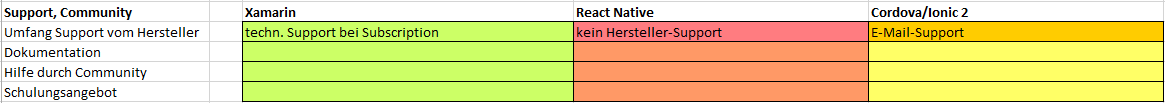
\includegraphics[width=1\textwidth]{Bilder/Auswertung_SupportCommunity.PNG}
	\caption{Bewertungsmatrix Kategorie Support und Community}
	\label{fig:AuswSuppComm}
\end{figure}

Beim Xamarin Framework wird ein technischer Support mit Erwerb einer Subscription angeboten. Zudem bekommen alle Kunden, die mindestens die 'Professional'-Version des Frameworks käuflich erworben haben einen E-Mail-Support\footcite{XamarinPricing}. 
\\
Auf der Homepage von Xamarin ist im 'Developer Center' eine ausführliche Dokumentation inklusive API-Spezifikation zu finden. Zusätzlich hat man dort Zugriff auf Guides zu verschiedenen Funktionalitäten und Thematiken mit Beispielen und Code-Rezepten\footcite{XamarinHomepage}. Allein auf GitHub stehen über 13.500 öffentliche Repositories zur Verfügung\footcite{GitHubTrending}. Zusätzlich hat man noch Zugriff auf ein FAQ, welches bei gängigen Problemen mit der Installation und Entwicklung mit Xamarin hilft\footcite{XamarinHomepage}. 
\\
Xamarin betreibt ein eigenes Forum mit mehreren Unterforen zu Themen wie Android, iOS, Tools etc. Es befinden sich über 80.000 Threads mit über 400.000 Posts in diesem Forum (Stand Februar 2017)\footcite{XamarinForums}. Zusätzlich zum Xamarin Forum sind bei der 'Stack Overflow'-Community\footcite{StackOverfolw} noch über 55.000 Threads, die sich mit Themen zu Xamarin beschäftigen, zu finden. 
\\
Was Schulungen betrifft, so bieten die 'Xamarin Consulting Partners' sowohl Präsenz- als auch Videokonferenz-Schulungen an. Eine Präsenzschulung kann für 2-10 Tage gebucht werden und kostet dabei 1500\$ pro Tag plus Reisekosten. Schulungen via Konferenzschaltung können für 2-6 Stunden gebucht werden und kosten 200\$ pro Stunde. Neben diesen Schulungen bietet Xamarin auch Video Tutorials und Webinare an\footcite{XamarinHomepage}. 
\\
\\
Ionic bietet allen Kunden, die mindestens die 'Business'-Version käuflich erworben haben, einen E-Mail-Support an\footcite{IonicHomepage}. 
\\
Ähnlich zum Xamarin 'Developer Center' bietet auch Ionic eine umfangreiche Dokumentation mit API Spezifikation an. Guides zu verschiedensten Themen wie 'Third Party Libraries' und einzelne Anwendungsfunktionalitäten, sowie Video-Crash-Kurse sind ebenfalls auf der Homepage von Ionic zu finden. Besonders ausführlich ist die große Übersicht sämtlicher verfügbarer UI-Elemente. Zu jedem UI-Element ist Beispielcode hinterlegt und auf einem eingeblendeten Emulator kann man sich jedes Element in den 3 Versionen iOS, Android und Windows Phone ansehen. Beispielcode und Links zu GitHub-Repositories zu einzelnen Funktionalitäten sind ebenfalls vorhanden. Zusätzlich bietet Ionic, wie Xamarin auch, ein FAQ an\footcite{IonicHomepage}. 
\\
Ionic betreibt ein eigenes Forum, indem sich bereits über 30.000 Threads zu verschiedenen Themen befinden\footcite{IonicForums}. Im 'Stack Overflow'-Forum\footcite{StackOverfolw} befinden sich weitere über 35.000 Threads über Ionic-bezogene Themen. Allerdings thematisieren nur knapp 7.000 Threads die Version Ionic 2. 
\\
Schulungen werden zwar keine von Ionic selbst angeboten, jedoch gibt es die sogenannten 'Trusted Partners'. Dies sind Unternehmen, die auf Anfrage bei der Umsetzung einer Ionic Anwendung unterstützen oder sogar die Implementierung komplett übernehmen. Auf der Homepage von Ionic gibt es zudem noch Buchempfehlungen und Links zu kostenpflichtigen eLearning-Kursen\footcite{IonicHomepage}.
\\
\\
Im Gegensatz zu den Frameworks Xamarin und Ionic bietet React Native keinen Hersteller-Support wie E-Mail-Support oder ähnliches an.
\\
Was den Umfang der Dokumentation anbelangt, so bietet auch React Native Erläute-rungen und Beispiel-Code zur Verwendung verschiedener Funktionalitäten, sowie eine API Spezifikation auf der Homepage an. Der Code vieler Plugins, die genutzt werden können, kann auf GitHub eingesehen werden. Auf der Homepage von React Native finden sich zudem noch Buchempfehlungen\footcite{ReactNativeHomepage}.
\\
React Native betreibt zwar kein eigenes Forum, es gibt dafür allerdings eine Facebook-Gruppe, in der über React Native-bezogene Themen diskutiert wird. In dieser Gruppe befinden sich über 12.500 Mitglieder (Stand Februar 2017)\footcite{ReactNativeFB}. Im 'Stack Overflow'-Forum\footcite{StackOverfolw} gibt es über 18.000 Threads mit React Native-bezogenen Themen. 
\\
Von React Native selbst werden keine Schulungen, Video-Kurse oder dergleichen angeboten. 

\section{Entwicklung} \label{AuswEntwicklung}

Die ausgefüllte Bewertungsmatrix für die Kategorie 'Entwicklung' ist in nachfolgender Abbildung \ref{fig:AuswEntw} dargestellt.

\begin{figure}[h]
	\centering
	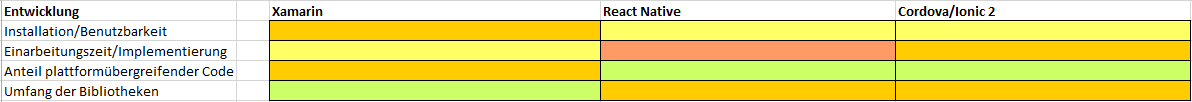
\includegraphics[width=1\textwidth]{Bilder/Auswertung_Entwicklung.PNG}
	\caption{Bewertungsmatrix Kategorie Entwicklung}
	\label{fig:AuswEntw}
\end{figure}

Hat man bereits ein Visual Studio installiert und möchte Xamarin integrieren, so ist dies nicht ohne Mehraufwand möglich. Einfacher ist es, Visual Studio direkt zusammen mit Xamarin zu installieren. Hierzu muss nur der Installer von der Xamarin Homepage heruntergeladen und ausgeführt werden. Alles Notwendige für die Entwicklung mit Xamarin ist bei der Installation von Visual Studio bereits vorausgewählt. Der Xamarin Installer installiert zusätzlich noch weitere benötigte Komponenten, wie ein Android SDK und NDK. Es muss keine weitere Software separat beschafft werden. Startet man nach der erfolgreichen Installation die IDE Visual Studio, so kann direkt mit der Entwicklung mit Xamarin gestartet werden, indem ein neues Projekt 'Android App' angelegt wird. Anders als bei der nativen Entwicklung mit Android Studio gibt es hier allerdings keine Design-Vorauswahl bei der Projekterstellung wie zum Beispiel einen \textit{NavigationDrawer} für die Navigation. Dafür gibt es sogenannte 'Pre Built Apps', das sind beispielhafte fertige Anwendungen, wie unter anderem Shopping- oder CRM-Anwendungen. 
\\
Auf der Xamarin Homepage\footcite{XamarinHomepage} findet sich einiges an Beispielcode zu verschiedensten Funktionalitäten. Viele dieser Beispielprojekte sind allerdings nicht direkt kompilierbar. Es ist immer aufwendiges recherchieren notwendig, welche Verweise, Components oder Einstellungen im Projekt angepasst werden müssen, da diese Informationen nicht mit angegeben sind. Für die Verwendung von zum Beispiel nativen UI-Elementen müssen sogenannte 'Components' installiert und dem Projekt hinzugefügt werden. Welche 'Components' für ein gewünschtes Feature benötigt werden muss selbst recherchiert werden. Bei der Auswahl dieser 'Components' gibt es oft Schwierigkeiten, da manche 'Components' zwingend in einer übereinstimmenden Version installiert sein müssen, um Versionskonflikte zu vermeiden. Welche 'Components' übereinstimmende Versionen haben müssen, kann nur durch Recherche oder Probieren ermittelt werden. Hierbei muss zusätzlich darauf geachtet werden, dass eventuell nicht in allen Versionen das gewünschte Feature enthalten ist.
\\
Xamarin Anwendungen werden, wie schon in Kapitel \ref{chpXamarin} erwähnt, mit der objektorientierten Programmiersprache C\# entwickelt. Da C\# vom Aufbau her Java sehr ähnlich ist, ist es für einen Android- oder Java-Entwickler keine große Umstellung. Die Projektstruktur einer Android-Anwendung mit Xamarin ist identisch mit der nativen Projektstruktur. Die Layout-Dateien können mit wenigen Anpassungen von einer nativen Android-Anwendung übernommen werden. Mit diesen Voraussetzungen ist das Portieren einer nativen Android-Anwendung nach Xamarin unkompliziert. Die API für Zugriffe auf Hardware wie Sensoren und Speicher wirkt wie eine 1 zu 1 Umsetzung der Android API. Viele Klassen heißen gleich oder sehr ähnlich. Auch die Verwendung deckt sich mit der nativen. Dies macht es zwar jedem Android-Entwickler leicht, sich in Xamarin einzuarbeiten, jedoch bedingt dies zugleich mit sich, dass eben diese Code-Abschnitte nicht plattformübergreifend nutzbar sind. Ein höherer Anteil an plattformübergreifenden Code kann mit der Nutzung von Xamarin.Forms erreicht werden, wobei dann auf native UI-Elemente verzichtet werden muss. Zum Umfang der von Xamarin zur Verfügung gestellten Bibliotheken ist zu sagen, das im Rahmen dieser Arbeit keine Android-Funktionalität gefunden wurden, die nicht mit Xamarin umsetzbar waren. 
\\
\\
Auf der Homepage von Cordova fand ich leider keine schrittweise Installationsanleitung, man musste sich von mehreren Stellen die Informationen, darüber, was an Software installiert werden muss, zusammensuchen. Auch die Installation selbst verlief nicht ganz reibungslos, da es immer wieder zu Problemen bezüglich Pfadangaben wie zum Beispiel das JAVA\_HOME-Verzeichnis kam. Unter dem 'Get Startet'-Abschnitt findet sich erst keine direkte Anleitung zum Aufbau und der Entwicklung von Anwendungen und Plugins mit Cordova. Es wird lediglich die Installation und das Erstellen eines Projektes erklärt. Die Projektstruktur wird nicht näher erläutert und es bleibt unklar an welcher Stelle sich Source-Dateien zu befinden haben. In den Tutorials wird nur aufgezeigt, welche Berechtigungen und Methoden für verschiedene Hardware-Nutzungen wie Beschleunigungssensor oder Kamera benötigt werden. Es gibt aber kein 'Rezept' für eine erste lauffähige Anwendung. Da für diese Arbeit allerdings nur fertige Cordova Plugins in einer Ionic Anwendung genutzt werden, fällt dieser Aspekt bei der Bewertung des Zusammenspiels von Cordova und Ionic nicht groß ins Gewicht. 
\\
Ist Cordova bereits installiert, gestaltet sich die Installation von Ionic denkbar einfach: es muss nur ein Befehl in einer Kommando-Shell ausgeführt werden. Eine Ionic  Anwendung kann mit jedem beliebigen Editor entwickelt werden. Dies bringt einerseits Freiheiten, andererseits gibt es nur bedingt eine Autovervollständigung und keine Code-Generierungsmöglichkeiten. Ionic bietet beim Erstellen einer neuen Anwendung direkt 2 Navigationselemente mit an: eine Tableiste und einen Navigation-Drawer. Ionic bietet für sämtliche UI-Elemente eine Übersicht mit Beispielcode. Für Zugriffe auf Hardware-Elemente wie Sensoren oder Kamera werden Cordova-Plugins installiert und der Anwendung hinzugefügt. Welches Plugin für welche Funktionalität benötigt wird ist auf der Homepage von Ionic beschrieben. Benötigte Berechtigungen müssen nicht manuell hinzugefügt werden. Wie schon beim Xamarin Framework sind leider auch bei Ionic einige Beispiele nicht direkt kompilierbar.
\\
Da das Ionic Framework in der Version 2 erst Januar 2017 erschienen ist\footcite{IonicHomepage}, gibt es noch nicht für alle Funktionalitäten Beispiele. Viele Beispiele beziehen sich noch auf das Ionic 1 Framework. Da in Ionic 2 nicht direkt in JavaScript, sondern in TypeScript entwickelt wird, sind viele Ionic 1 Beispiele nicht 1 zu 1 in Ionic 2 umsetzbar. TypeScript bringt im Gegensatz zu 'reinem' JavaScript auch objektorientierte Strukturen mit sich\footcite{TypeScript}. Die 'ionic-native'-Bibliothek stellt Klassen zur Verfügung, die die Funktionalitäten der Cordova-Plugins kapseln und so für eine Implementierung mit TypeScript nutzbar machen. Leider fehlen in dieser Bibliothek noch einige Sensoren, wie zum Beispiel der Näherungssensor. Man muss allerdings auch bei einer Ionic 2 Anwendung dadurch nicht gänzlich auf die Verwendung dieser Sensoren verzichten. Externe oder selbstgeschriebene Cordova-Plugins können weiterhin in die Anwendung integriert und genutzt werden. Auf diese Weise muss dann aber meist auf die Nutzung von TypeScript in diesen Teilen der Anwendung verzichtet und JavaScript verwenden werden. Die Benutzeroberfläche einzelner Seiten einer Anwendung wird in separaten HTML-Dateien erstellt. Anwendungen werden direkt für alle 3 Plattformen, Android, iOS und Windows Phone, implementiert. Je nachdem für welche Plattform die Anwendung am Schluss gebaut wird, werden die einzelnen UI-Elemente optisch automatisch angepasst. Der Anteil an plattformübergreifenden Code ist dadurch sehr hoch. Zum Umfang der existierenden Bibliotheken lässt sich sagen, dass leider vieles, besonders im Bereich der Sensor-Nutzung, noch nicht in der Ionic 2 API integriert ist. Dies macht die Verwendung einiger Funktionalitäten momentan noch umständlich. 
\\
\\
Die 'Get Startet'-Anleitung auf der React Native Homepage\footcite{ReactNativeHomepage} führt einen Schritt für Schritt durch die Installation über die Kommando-Shell bis zum Start einer ersten leeren Anwendung auf dem Testgerät. Wie auch bei dem Ionic Framework kann der Code einer React Native-Anwendung mit jedem beliebigen Editor geschrieben werden. Erstellt werden die Anwendungen über eine Kommando-Shell. Auf viele Vorzüge einer Entwicklung in einer IDE wie Android Studio oder Visual Studio muss auch hier verzichtet werden. Bei der Erstellung einer neuen Anwendung gibt es bei React Native leider keine vorgefertigten Navigationselemente. Dafür bietet die Ionic Homepage ausführliche und hilfreiche Guides für die Integration und Verwendung verschiedener Navigationselemente. Sowohl im 'Get Startet'-Tutorial, wie auch bei vielen Beispielen ist nicht ersichtlich, wo in der Projektstruktur der Anwendung die Quelldateien liegen, beziehungsweise liegen sollen. Es scheint vorausgesetzt zu werden das man weiß, wie die Projektstruktur aufgebaut ist. Für Zugriffe auf Hardware-Komponenten werden ähnlich wie bei Ionic Plugins installiert und in die Anwendung integriert. Auch hier ist es in den meisten Fällen nicht notwendig Berechtigungen manuell in das \textit{Android Manifest} einzutragen. Plugins können wie bei Ionic auch selbst geschrieben werden. Wie bei den anderen Frameworks sind auch viele Beispiele, die auf der Homepage des Frameworks verfügbar sind, nicht direkt kompilierbar. Oft werden benötigte Importe nicht mit angegeben. Einige Beispiele waren selbst nach stundenlanger Fehlersuche nicht lauffähig. Hier ist eine beobachtete Ursache die, dass die Beispiele für frühere Versionen von React Native erstellt wurden und in der aktuellen Version nicht mehr kompilierbar sind. Die Suche nach brauchbaren Beispielen gestaltete sich insgesamt mühsamer als bei Xamarin und Ionic.
\\
Eine React Native Anwendung wird JSX programmiert, eine JavaScript-Erweiterung mit objektorientierten Elementen\footcite{JSX}. Leider stellt das React Native Framework nur wenige an die native Benutzeroberfläche angelehnten UI-Elemente zur Verfügung. Einzelne Elemente müssen über \textit{styles} angepasst werden, um native UI-Elemente der einzelnen Plattformen nachzubilden. Positiv zu vermerken ist dabei allerdings, dass der Entwickler über die hohe Anpassbarkeit der UI-Elemente viele Freiheiten hat was das Design der Anwendung betrifft. Die UI-Elemente werden mittels integriertem HTML-Code innerhalb der Quelldateien und innerhalb der JSX-Klassen implementiert. Dies lässt dem Entwickler zwar viel Spielraum was das Code-Design betrifft, macht den Code dafür allerdings auch schnell unübersichtlich. Wie schon mit Ionic wird auch mit React Native eine Anwendung direkt für alle Plattformen geschrieben. Der Anteil an plattformunabhängigen Code ist vergleichbar mit dem von Ionic. Der Umfang an existierenden Bibliotheken lässt sich in dem begrenzten Rahmen der für diese Arbeit genutzten und recherchierten Funktionalitäten mit dem für das Ionic 2 Framework vergleichen.


\section{Hersteller}

Nachfolgende Abbildung \ref{fig:AuswHerst} zeigt den Abschnitt 'Hersteller' der ausgefüllten Bewertungsmatrix.

\begin{figure}[h]
	\centering
	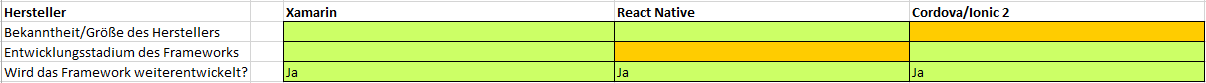
\includegraphics[width=1\textwidth]{Bilder/Auswertung_Hersteller.PNG}
	\caption{Bewertungsmatrix Kategorie Hersteller}
	\label{fig:AuswHerst}
\end{figure}

Wie man vielleicht schon anhand der engen Verknüpfung des Xamarin Frameworks mit der IDE 'Visual Studio' vermuten könnte, so steht hinter Xamarin Inc. der Hard-ware- und Software-Hersteller 'Microsoft'. Das Xamarin Framework befindet sich aktuell (Stand Februar 2017) in der Major-Version 'Cycle 9'. Es werden regelmäßig wöchentlich Releases herausgegeben. Die aktuellste unterstützte Android-Version ist die Version 7.1, welche auch die aktuellste Android-Version ist (Stand Februar 2017). Die aktuellste iOS-Version, für die mit dem Xamarin Framework entwickelt werden kann, ist die Version 10.4. Das Framework wird weiterentwickelt\footcite{XamarinHomepage}. 
\\
\\
Hinter dem Cordova-Framework steht der Software-Hersteller Apache. Das Ionic Framework ist das einzige Produkt des Unternehmens Drifty. Die Version 2 des Ionic Frameworks wurde am 25.01.2017 veröffentlicht. Sowohl vom Ionic Framework als auch vom Cordova Framework werden mehrere Releases pro Monat mit Neuerungen und Bugfixes herausgebracht. Beide Frameworks werden weiterentwickelt\footcite{Cordova}. 
\\
\\ 
Herausgeber des React Native Frameworks sind die Unternehmen Facebook und Instagram. Das Framework befindet sich aktuell (Stand Februar 2017) in der Version 0.42. Es befindet sich somit noch in einer Beta-Version. Entwicklern wird die Möglichkeit geboten sogenannte 'Feature Requests' zu stellen. Requests, die von ge-nügend Entwicklern gewünscht werden, werden in die Planung der weiteren Entwicklung mit aufgenommen. Auf der Homepage des React Native Frameworks kann man einsehen, welche 'Feature Requests' sich momentan in der Umsetzung befinden. Seit Beginn 2017 werden zudem regelmäßige monatliche Releases veröffentlicht\footcite{ReactNativeHomepage}. 

\section{OS-Versionen}

Die Bewertung der einzelnen Frameworks in der Kategorie 'OS-Versionen' ist in nachfolgender Abbildung \ref{fig:AuswOSVersionen} dargestellt.
\clearpage

\begin{figure}[h]
	\centering
	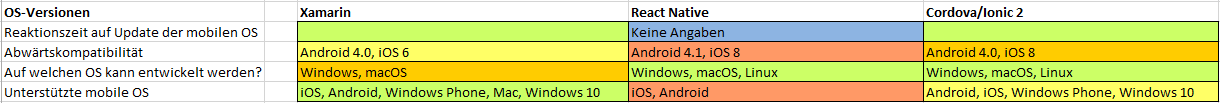
\includegraphics[width=1\textwidth]{Bilder/Auswertung_OSVersionen.PNG}
	\caption{Bewertungsmatrix Kategorie OS-Versionen}
	\label{fig:AuswOSVersionen}
\end{figure}

Zwischen dem Android-Update auf die Version 7.1 am 4.10.2016 und dem Update des Xamarin Frameworks für die Android-Version 7.1 am 19.10.2016 lagen nur knapp mehr als 2 Wochen\footcite{XamarinHomepage}.
\\
Mit dem Framework Xamarin kann auf Windows-Systemen ab Windows 7 und auf Apple-Computern ab der Betriebssystem-Version OS X El Capitan (10.11) entwickelt werden. Anwendungen können für die Systeme iOS, Android, Windows Phone, Mac und Windows 10 geschrieben werden\footcite{XamarinHomepage}. 
\\
Zur Abwärtskompatibilität lässt sich sagen, dass mit dem Xamarin Framework für Android-Geräte ab Version 4.0, für Apple-Geräte ab Version iOS6 und für Windows Phone ab Windows Phone 7 entwickelt werden kann. Bei Windows Phone 7-Anwen-dungen muss allerdings auf die Verwendung von Xamarin.Forms verzichtet werden\footcite{XamarinHomepage}.
\\
\\
Was die Reaktionszeit auf ein Update der mobilen Betriebssysteme anbelangt, ist bei der Kombination von Ionic und Cordova Cordova der entscheidende Faktor, da API-Zugriffe bei Ionic-Anwendungen hauptsächlich über Cordova-Plugins realisiert werden. Die Reaktionszeit von Apache Cordova war beim letzten Android-Update vom 4.10.2016 nur einen Tag länger als die des Xamarin Frameworks. Cordova wurde am 20.10.2017 für die Android-Version 7.1 geupdatet\footcite{Cordova}.
\\
Sowohl mit Ionic als auch mit Cordova kann auf den Systemen Windows, Linux und OS X entwickelt werden. Ionic-Anwendungen können für die Betriebssysteme Android, iOS, Windows Phone und Windows 10 geschrieben werden\footcite{IonicHomepage}. Cordova-Anwendungen und -Plugins können zudem auch für die Systeme Bada, Blackberry, Firefox OS, Symbian, Tizen, webOS und Ubuntu Touch entwickelt werden\footcite{Cordova}. 
\\
Was die Abwärtskompatibilität betrifft, so unterstützen Ionic und Cordova Android ab der Version 4.0, iOS ab Version iOS 8, Windows Phone ab Windows Phone 8.1 und Windows ab Windows 8.1. Cordova unterstützt zudem noch Blackberry ab Version 4.6, OS X ab Version 10.9 und Ubuntu ab Version 14.04\footcite{Cordova}\footcite{IonicHomepage}. 
\\
\\
Bei dem Framework React Native war die Reaktionszeit auf ein Update der mobilen Betriebssysteme betrifft leider nicht aus den Release Notes ablesbar, es konnten keine Angaben gefunden werden. Mit dem React Native Framework kann auf Apple-Computern, Windows-PCs und Linux-Rechnern entwickelt werden. React Native-Anwendungen laufen auf den beiden mobilen Betriebssystemen iOS und Android. Auf einem Android-Gerät muss dabei mindestens Version 4.1 und auf einem Apple-Gerät mindestens Version 8.0 installiert sein\footcite{ReactNativeHomepage}. 

\section{Funktionsumfang} \label{AuswFunktion}

Die ausgefüllte Bewertungsmatrix für die Kategorie 'Entwicklung' ist in nachfolgender Abbildung \ref{fig:AuswFunktion} dargestellt.

\begin{figure}[h]
	\centering
	\includegraphics[width=1\textwidth]{Bilder/Auswertung_Funktionsumfang.PNG}
	\caption{Bewertungsmatrix Kategorie Funktionsumfang}
	\label{fig:AuswFunktion}
\end{figure}

Wie schon in Kapitel \ref{AuswEntwicklung} erwähnt, bietet die API von Xamarin Zugriff auf alle Funktionalitäten, die eine native Android Anwendung auch bietet. Alle Sensoren können ausgelesen werden, Kommunikation via WiFi und Bluetooth ist möglich und eine mit Xamarin geschriebene Anwendung kann Notifications auslösen. Zudem kann auf die native Kamera-Anwendung von Android zugegriffen werden, die alle gebräuchlichen Kamerafunktionen wie Blitz und Kamerawechsel integriert hat. Dateien wie Fotos können an verschiedenen Speicherorten des Smartphones abgelegt werden. 
\\
\\
Bei der Kombination der Frameworks Cordova mit Ionic 2 fehlen noch Schnittstellen zu Barometer-, Näherungs- und Umgebungslichtsensor-Plugins in der Ionic 2 \textit{native}-Bibliothek. Wie schon in Kapitel \ref{AuswEntwicklung} beschrieben, können trotzdem mit Mehraufwand Plugins eingebunden werden, die diese Sensoren ansprechen können. Wie bei dem Xamarin Framework kann auch mit Ionic die native Android Kamera-Anwendung in die eigene Anwendung integriert werden. Kommunikation via WiFi und Bluetooth sowie Zugriffe auf das Dateisystem und Notifications sind ebenfalls möglich. 
\\
\\
Außer der Nutzung des Barometers, zu der keine Informationen gefunden wurden, ist das Auslesen aller anderer in der Bewertungsmatrix (Abbildung \ref{fig:AuswFunktion}) gelisteten Sensoren mit dem React Native Framework umsetzbar. Sowohl auf die Front- als auch auf die Rückkamera eines Smartphones kann zugegriffen werden. Allerdings ist ein Aufruf der nativen Android-Kameraanwendung nicht in der API des Frameworks integriert, so muss eine Kameraanwendung mit allen Einstellungsmöglichkeiten selbst implementiert werden. Wie schon bei Xamarin und Ionic sind auch mit React Native Kommunikation via Bluetooth und Wifi sowie auch Notifications möglich. 
\clearpage

\section{GUI-Design} \label{AuswGUI}

Nachfolgende Abbildung \ref{fig:AuswGUI} zeigt den Abschnitt 'GUI-Design' der ausgefüllten Bewertungsmatrix.

\begin{figure}[h]
	\centering
	\includegraphics[width=1\textwidth]{Bilder/Auswertung_GUI.PNG}
	\caption{Bewertungsmatrix Kategorie GUI-Design}
	\label{fig:AuswGUI}
\end{figure}

Bei der Entwicklung mit Xamarin bietet die IDE 'Visual Studio' einen GUI-Designer zum Zusammenstellen der Benutzeroberfläche jeder Seite der Anwendung. Allerdings ist die Auswahl der verfügbaren UI-Elemente sehr begrenzt und es stehen zum Beispiel keine Elemente im Android 'Material Design' zur Verfügung. Außerhalb der Nutzung des GUI-Designers können alle nativen Android UI-Elemente mit dem Xamarin-Framework verwendet werden. 'Visual Studio' bietet für das Testen der Anwendung einen eigenen Emulator. Dadurch, dass sämtliche nativen UI-Elemente mit Xamarin nutzbar sind, ist eine 1 zu 1 Umsetzung einer nativen Benutzeroberfläche möglich. Für die Unterstützung beim GUI-Design konnte dem Xamarin-Framework keine gute Benotung gegeben werden, da zum einen, wie oben erwähnt, der GUI-Designer nur sehr beschränkt nutzbar ist und zum anderen die Verwendung vieler nativer UI-Elemente aufwändig recherchiert werden musste. 
\\
\\
Ionic bietet für die Entwicklung der Benutzeroberfläche keinen GUI-Designer an, alles muss manuell in HTML implementiert werden. Die nativen Android UI-Elemente können bei der Entwicklung mit Ionic zwar nicht verwendet werden, dafür gibt es ein großes Angebot UI-Elementen, die den originalen 'Material Design'-Elementen sehr nahe kommen. Die gewählten UI-Elemente passen sich, sobald die Anwendung gegen ein bestimmtes Betriebssystem wie Android kompiliert wurde, dem entsprechenden Design an. Die Große Auswahl an UI-Elementen ermöglicht das Design einer Benutzeroberfläche, die einer nativen sehr ähnlich sein kann. Ionic selbst bietet zwar keinen Emulator zum Testen der Anwendung, es kann aber der Android Emulator des 'Android Studios' verwendet werden. Trotz fehlendem GUI-Designer ist die Unterstützung beim GUI-Design umfangreich durch eine Galerie sämtlicher zur Verfügung stehender UI-Elemente plus Beispielcode auf der Homepage von Ionic gegeben. 
\\
\\
Wie schon bei Ionic, steht auch bei der Entwicklung mit React Native kein GUI-Designer zur Verfügung. Man hat keinen Zugriff auf die nativen UI-Elemente, aber es gibt eine große Auswahl an UI-Elementen mit einem hohen Maß an Anpassbarkeit (siehe Kapitel \ref{AuswEntwicklung}). Auf diese Weise ist auch mit dem React Native Framework eine Benutzeroberfläche umsetzbar, die der nativen nicht unähnlich ist. Sie weicht allerdings deutlicher vom Original ab als die Ionic-Variante. Zudem ist auch die Unterstützung beim GUI-Design vergleichbar schlechter, aber nicht so mühsam wie mit dem Xamarin-Framework. Möchte man seine Anwendung mit einem Emulator testen, so kann der Android Emulator des 'Android Studio' verwendet werden. React Native bietet keinen eigenen Emulator an, die Anwendung kann dafür im Browser getestet werden. 

\section{Interoperabilität} \label{AuswInterop}

Die Bewertung der einzelnen Frameworks in der Kategorie 'Interoperabilität' ist in nachfolgender Abbildung \ref{fig:AuswInterop} dargestellt.

\begin{figure}[h]
	\centering
	\includegraphics[width=1\textwidth]{Bilder/Auswertung_Interoperabilitaet.PNG}
	\caption{Bewertungsmatrix Kategorie Interoperabilität}
	\label{fig:AuswInterop}
\end{figure}

Mit dem Xamarin Framework sind Webservice-Aufrufe umsetzbar und Drittanbieter-Bibliotheken können laut Xamarin in eine Anwendung eingebunden werden. Möchte man für seine Entwicklung das Xamrin Framework einsetzen, so muss auf einem Windows-PC mit der IDE 'Visual Studio' gearbeitet werden. Auf einem Apple-Com-puter ist das 'Xamarin-Studio' verpflichtend. Support-Tools sind vorhanden. 
\\
\\
Auch mit der Kombination von Ionic und Cordova sind Webservice Aufrufe umsetzbar mit zum Beispiel SOAP web Services. Drittanbieter-Bibliotheken können via \textit{npm} eingebunden werden. Für die Entwicklung gibt es keine vorgeschriebene IDE, es kann mit einem Text-Editor nach Wahl programmiert werden. Support-Tools sind ebenfalls vorhanden, wie zum Beispiel die Ionic Cloud. Mit der Ionic Cloud sind unter anderem Updates vorbei am App Store und das Umwandeln des Ionic Codes in native Binaries für verschiedene Plattformen möglich. 
\\
\\
Auch mit dem React Native Framework lassen sich Webservice-Aufrufe realisieren. Hier hat man einmal die Möglichkeit den \textit{react-native-web-service-handler} über \textit{npm} zu installieren und für die Umsetzung von Webservice-Aufrufen zu nutzen oder man benutzt die \textit{XMLHttpRequestAPI} aus der \textit{react-native}-Bibliothek. Es gibt 2 Typen von Drittanbieter-Bibliotheken, die integriert werden können: einmal native Module und JavaScript Module. Wie auch bei der Entwicklung mit dem Ionic Framework kann man für die Entwicklung mit dem React Native Framework einen beliebigen Texteditor verwenden. Was Support-Tools angeht, konnte nichts ermittelt werden.

\section{Tests}

Die ausgefüllte Bewertungsmatrix für die Kategorie 'Tests' ist in nachfolgender Abbildung \ref{fig:AuswTest} dargestellt.

\begin{figure}[h]
	\centering
	\includegraphics[width=1\textwidth]{Bilder/Auswertung_Tests.PNG}
	\caption{Bewertungsmatrix Kategorie Tests}
	\label{fig:AuswTest}
\end{figure}

Xamarin bietet automatisierte Tests in einer Test-Cloud ab 99\$ pro Monat an. Für diesen Preis kann allerdings nur auf einem Gerät gleichzeitig für eine 'Device Hour' getestet werden. Möchte man simultan auf mehreren Geräten testen, so ist dies für einen Aufpreis auch möglich. Eine 'Device Hour' bezeichnet dabei die Zeit, die Tests auf Testgeräten laufen. Zum Beispiel entsprechen 5 min Testen auf 5 Geräten gleichzeitig 25 'Device Minutes'. Für das Schreiben automatisierter Tests, mit denen dann in der Test Cloud getestet werden kann, bietet Xamarin das Test Framework namens 'Calabash' an\footcite{XamarinHomepage}. 
\\
\\
Ionic bietet Live Browser Tests für die Entwicklung von Ionic Anwendungen an. Die im Browser dargestellte Anwendung wird dabei automatisch geupdatet, sobald etwas am Code geändert wurde. Ionic bietet keine speziellen Tools für die Generierung von Tests an\footcite{IonicHomepage}. 
\\
\\
Das React Native Repository stellt verschiedene Jest Tests zur Verfügung, die via \textit{npm} in einer Kommando-Shell ausgeführt werden können. Jest Tests sind JavaScript-Only Tests. Für React Native Android Anwendungen können Unit Tests geschrieben und ausgeführt werden und sowohl für Android als auch iOS sind Integrationstests möglich\footcite{ReactNativeHomepage}. 

\section{Performance}

\begin{tabular}{lllll}
\textbf{Framework} & \textbf{Kamera öffnen} & \textbf{Bild speichern} & \textbf{Sensordaten lesen} & \textbf{Galerie laden}\\
nativ & 1 & 1 & 1 & 1\\
Xamarin & 1 & 1 & 1 & 1\\
Ionic & 1 & 1 & 1 & 1\\
React Native & 1 & 1 & 1 & 1\\
\end{tabular}



\section{Programmiersprache}

Nachfolgende Abbildung \ref{fig:AuswProgr} zeigt den Abschnitt 'Programmiersprachen' der ausgefüllten Bewertungsmatrix.

\begin{figure}[h]
	\centering
	\includegraphics[width=1\textwidth]{Bilder/Auswertung_Programmiersprachen.PNG}
	\caption{Bewertungsmatrix Kategorie Programmiersprachen}
	\label{fig:AuswProgr}
\end{figure}

Xamarin-Anwendungen werden in C\# und Ionic und React Native Anwendungen in JavaScript implementiert. Wobei erwähnenswert ist, dass Ionic 2 die auf JavaScript basierende Sprache TypeScript und React Native die Abwandlung JSX von JavaScript verwendet. Layouts werden bei allen 3 Frameworks in HTML implementiert.  

\section{Sicherheit}

Die Bewertung der einzelnen Frameworks in der Kategorie 'Sicherheit' ist in nachfolgender Abbildung \ref{fig:AuswSicherheit} dargestellt.

\begin{figure}[h]
	\centering
	\includegraphics[width=1\textwidth]{Bilder/Auswertung_Sicherheit.PNG}
	\caption{Bewertungsmatrix Kategorie Sicherheit}
	\label{fig:AuswSicherheit}
\end{figure}

Im Bereich Sicherheit wurde bei der Entwicklung mit den Frameworks Xamarin, Ionic mit Cordova und React Native festgestellt, dass alle Frameworks das native Rechtemanagement unterstützen und Berechtigungen wie bei nativen Android-Anwen-dungen im \textit{Android Manifest} erteilt werden. VPN Verbindungen können ebenfalls mit allen getesteten Frameworks umgesetzt werden. 